\chapter{Requirements}
In the first part of the chapter we focus on the analysis of creating wholesome solution for taxi company and related business requirements. In the second part we specify requirements from the technical point of view - whether back-end or cooperating front-end. In the end we specify individual parts of back-end application and what they should fullfill.
\section{Business requirements  \todo{JUST DRAFT! write in sentences, structure it}} 
\begin{itemize}
	\item Handle order system - staff fluctuation is high, train employees is expensive - especially dispatchers, which must have good estimate
	\item Allow customers to order directly via their phone apps or other sources - saving costs of dispatching. Because it is very easy to order via phone call make it as easy as possible
	\item Customers must have overview how much their order will approximetly cost and must be able to select their driver. Also they must have approximate estimate when their taxi will come.
	\item Customers should be informed about their ordered driver status - where he is and when them will come
	\item better customer service - remember name, favorite location, other things
	\item security - strong competition, already few cases of hacking and data stealing
	\item some of the things written tailored for our local taxi company but should be easily rewritten and reused for some other company with differnet requirements and priorities
	\item predicted data size for the project for now: 10 drivers - 7 online, 7 cars, 10 dispatchers - 2 online, 6000 customers, 800 orders per week
	\item authorization
	\item two main types of orders - scheduled on time and normal. Our high priority is to be there for scheduled precisely on time.
	\item handling frauds
\end{itemize}
\section{Technical requirements}
\begin{itemize}
	\item Separate back-end and frontend - allows more customization on frontend which can and will change more frequently totally independently on backend. On frontend - where are apps and PWAs and orders through FB messenger for example.
	\item HTTPS
	\item Frontend-developer friendly instalation and independency
	\item Able to install easily on new server with possibility to scale - at least preparation
	\item Errors logging and alerting
\end{itemize}
\section{Back-end application requirements}

Based on the business requirements we decided that the back-end part of the application must take these five divisions into account: Customers, Employees, Vehicles, Orders and Noticications. In the rest of the chapter we are describing features that these modules should have.
\subsection{Customers}
Customers are uniquely identified by telephone number. It should support these operations:
\begin{itemize}
	\item Create and confirm
	\item Update
	\item Destroy
	\item Recover password
	\item Login and logout
	\item List favorite locations
	\item List all customers and show specific customer
\end{itemize}
\subsubsection{Operation create}
There are two ways how customer can be created. It is either directly through registration or indirectly by creating new order.

Directly registered customers has their own account to which they can login with password. Before they can do so, they must go through telephone number confirmation process - via sending sms with registration token. These accounts are used for orders directly from the customers via app.

Indirectly registered users exists mainly for better customer support. Most of them are created during telephone order by dispatchers.
\subsubsection{Operation update}
\subsubsection{Operation password recovery}
\subsubsection{Operation login and logout}
\subsubsection{Operation list favorite locations}
\subsubsection{Operation list all customers and show specific customer}

\subsection{Employees}
There three types of employees - admins, dispatchers and drivers.
\begin{itemize}
	\item driver locations
	\item shifts
\end{itemize}
\subsection{Vehicles}

\subsection{Orders}

\begin{figure}[h]\centering
	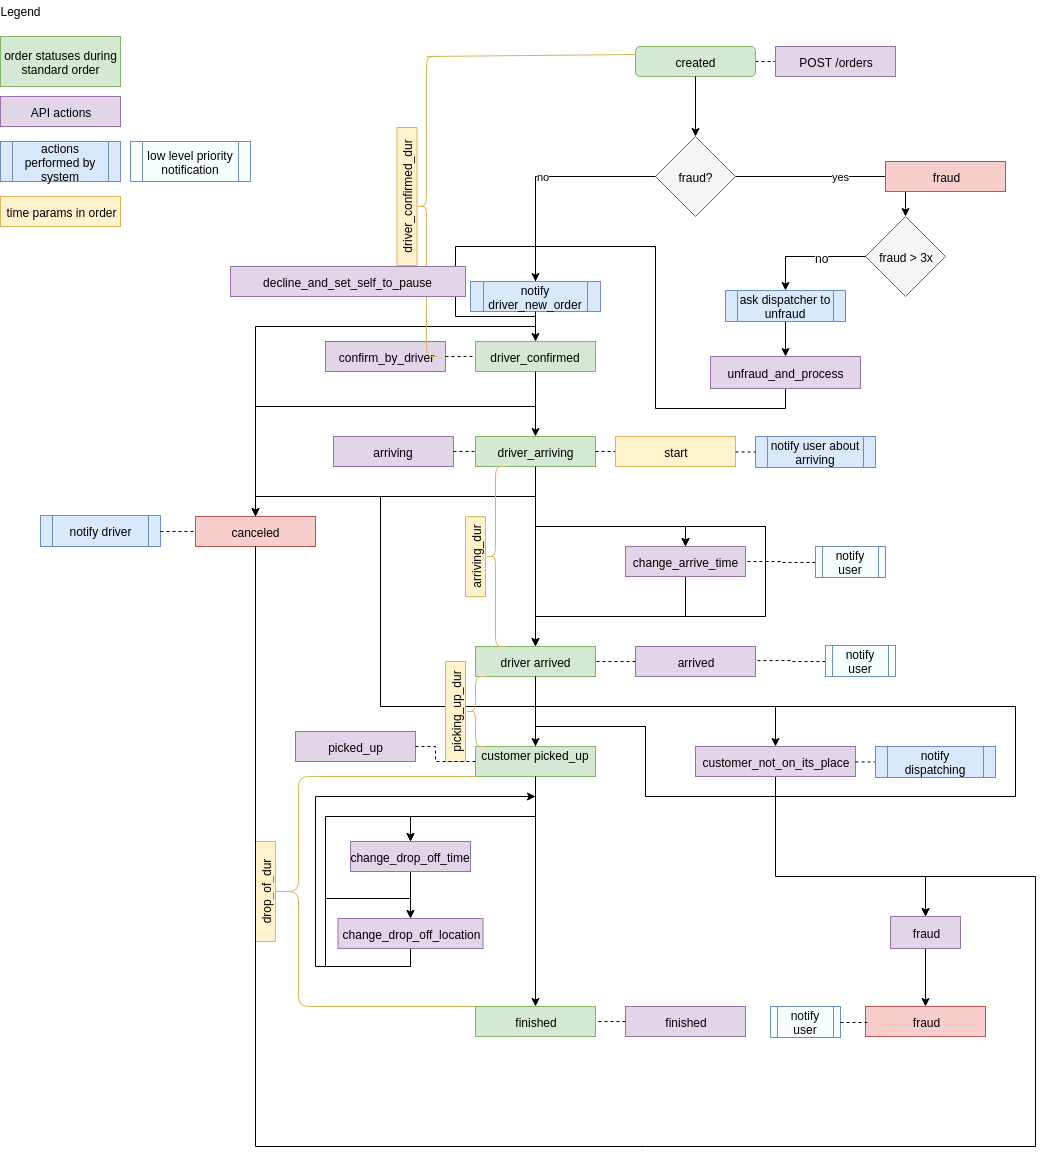
\includegraphics[width=\textwidth]{orders/order_process_scheme.png}
	\caption{Order process scheme}\label{order-process-scheme}
\end{figure}

\begin{figure}[h]\centering
	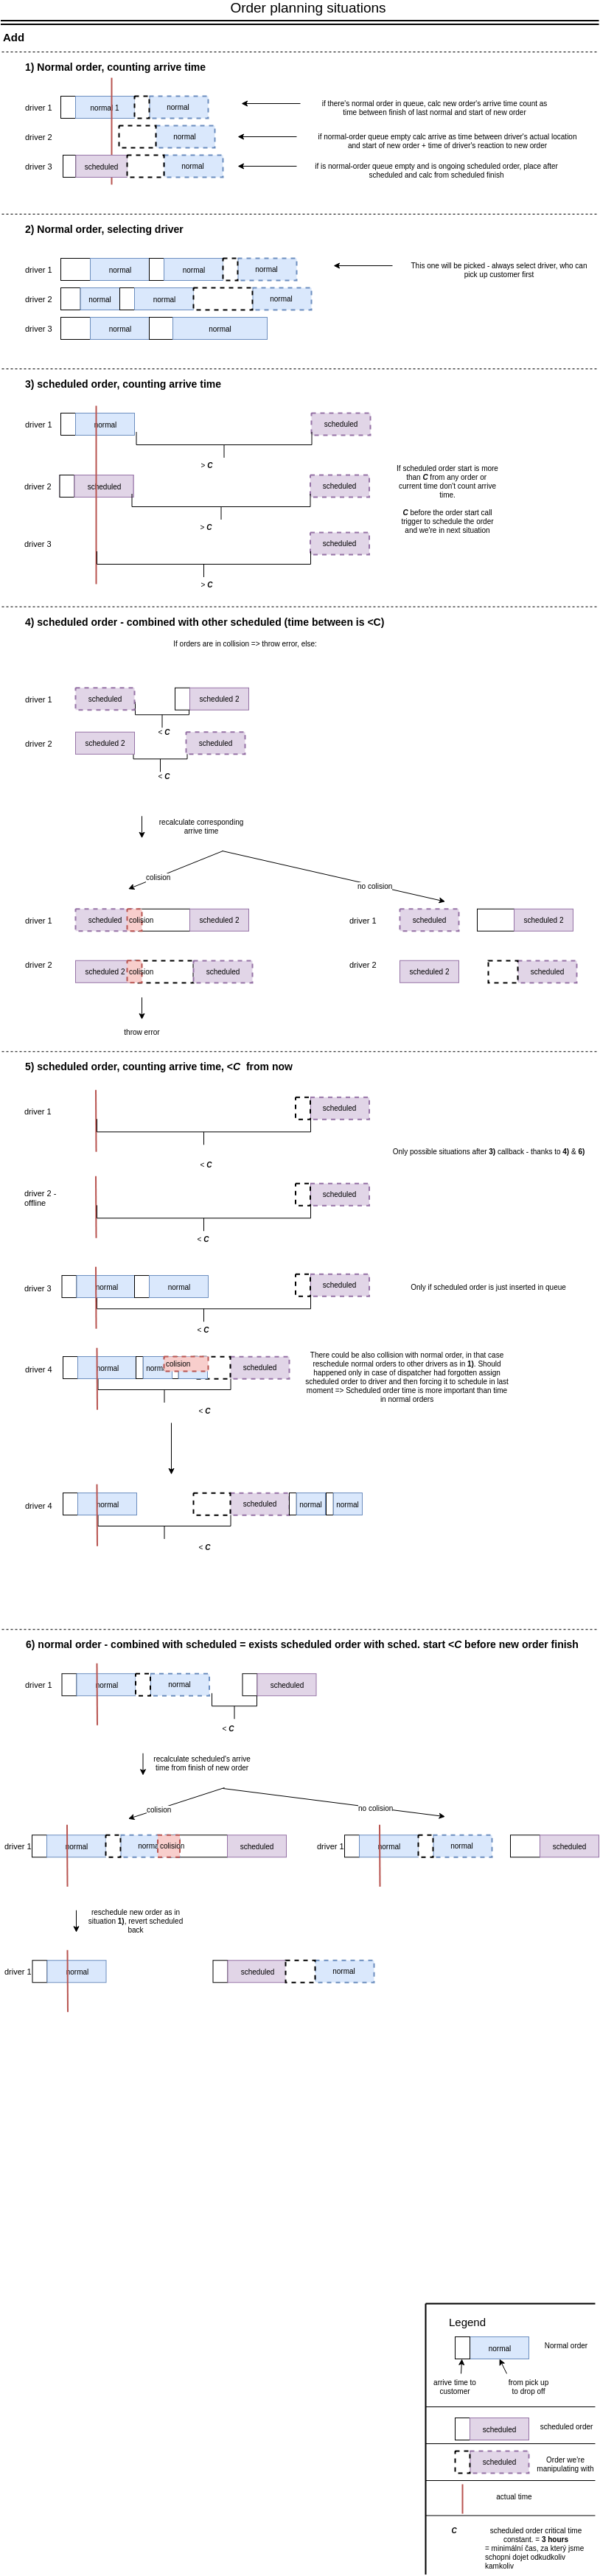
\includegraphics[scale=0.2	]{orders/order_planning.png}
	\caption{Order planning situations}\label{order-process-scheme}
\end{figure} 
\subsection{Notifications}
